\documentclass[conference,a4paper]{IEEEtran}
\IEEEoverridecommandlockouts

\usepackage[utf8]{inputenc}
\usepackage[T1]{fontenc}
\usepackage{cite}
\usepackage{amsmath,amssymb,amsfonts}
\usepackage{graphicx}
\usepackage{textcomp}
\usepackage{xcolor}
\usepackage{url}
\usepackage{array}
\usepackage{booktabs}
\usepackage{placeins}

\def\BibTeX{{\rm B\kern-.05em{\sc i\kern-.025em b}\kern-.08em
T\kern-.1667em\lower.7ex\hbox{E}\kern-.125emX}}

\begin{document}

\title{Semi-Supervised White Blood Cell Detection with Limited Bounding Box Annotations}

\author{
\IEEEauthorblockN{Fadime Yal\c{c}\i n}
\IEEEauthorblockA{
\textit{Department of Electrical and Computer Engineering} \\
\textit{Abdullah G\"ul University} \\
Kayseri, T\"urkiye}
}

\maketitle

\begin{abstract}
Automated white blood cell (WBC) detection in peripheral blood smear images is an important preprocessing step for digital hematology workflows. However, training object detection models requires bounding box annotations, which are costly and time-consuming to obtain in medical imaging. This study investigates whether semi-supervised object detection can improve WBC localization under limited annotation conditions. Using the TXL-PBC dataset, the task was formulated as single-class WBC detection by retaining only WBC bounding boxes. Four annotation settings were evaluated: 1\%, 5\%, 10\%, and 20\% of the training set were treated as labeled, while the remaining training images were treated as unlabeled. A Faster R-CNN detector was used as the supervised baseline, and two semi-supervised strategies were implemented: a STAC-inspired offline pseudo-labeling framework and a Soft Teacher-inspired exponential moving average teacher-student framework. Fixed and adaptive confidence thresholding strategies were also compared. In addition to mAP values, final detection precision, recall, and F1-score were reported, and pseudo-label quality was evaluated separately. The results showed that the supervised Faster R-CNN baseline already achieved high mAP@0.5 even at 1\% labeled data. STAC produced stable pseudo-labels across annotation ratios, while Soft Teacher with adaptive thresholding improved localization quality at 10\% and 20\% labeled data but was unstable in the 1\% and 5\% regimes. These findings indicate that pseudo-label quality analysis is essential for understanding semi-supervised detection under extreme annotation scarcity.
\end{abstract}

\begin{IEEEkeywords}
white blood cell detection, semi-supervised object detection, pseudo-labeling, Faster R-CNN, STAC, Soft Teacher, TXL-PBC
\end{IEEEkeywords}

\section{Introduction}
Peripheral blood smear examination is widely used in hematology because it provides visual information about blood cell morphology, distribution, and abnormal cellular patterns. In automated digital hematology systems, detecting white blood cells (WBCs) is a fundamental step before cell classification, counting, morphological scoring, or clinical decision support. If WBC localization is inaccurate, subsequent analysis stages may be negatively affected because missed or poorly localized cells can propagate errors to downstream models.

Deep learning-based object detection methods have achieved strong performance in medical image analysis. However, their success usually depends on the availability of accurately annotated training data. For object detection, this requirement is more demanding than image-level classification because each target object must be localized using a bounding box. In peripheral blood smear images, annotation requires careful visual inspection and may require expert knowledge, especially when cells overlap, appear near image borders, or show staining and illumination variations.

Semi-supervised object detection (SSOD) is a promising strategy for reducing annotation cost. Instead of relying only on a fully labeled dataset, SSOD uses a small labeled subset and a larger unlabeled subset. A teacher model first generates pseudo-labels on unlabeled images, and these pseudo-labels are then used to train or improve a student detector. Although SSOD methods have been studied extensively in general computer vision benchmarks, their behavior on small and specialized medical datasets is less clear. Medical datasets can introduce additional challenges such as limited visual diversity, annotation noise, and overconfident predictions under low-data conditions.

This study focuses on the following research question: \textit{Can semi-supervised pseudo-labeling strategies improve WBC detection performance under limited bounding box annotations, and how does pseudo-label quality change across different annotation ratios?} To answer this question, this work evaluates WBC detection on the TXL-PBC dataset under 1\%, 5\%, 10\%, and 20\% labeled-data settings. Faster R-CNN is used as the supervised baseline. STAC-inspired and Soft Teacher-inspired semi-supervised frameworks are compared under identical splits and experimental settings.

The main contributions of this study are as follows:
\begin{itemize}
    \item A low-annotation WBC detection benchmark is constructed using 1\%, 5\%, 10\%, and 20\% labeled subsets of the TXL-PBC training partition.
    \item Faster R-CNN, STAC-inspired pseudo-labeling, and Soft Teacher-inspired teacher-student training are compared under identical dataset splits.
    \item Fixed and adaptive pseudo-label confidence thresholding strategies are evaluated.
    \item Final detection performance is reported using mAP, precision, recall, and F1-score.
    \item Pseudo-label quality is analyzed separately from final detection performance using precision, recall, and F1-score.
    \item The effect of annotation scarcity on pseudo-label noise, label starvation, and localization performance is discussed with quantitative results and representative failure cases.
\end{itemize}

\section{Related Work}

\subsection{Blood Cell Detection and Dataset Quality}
Automated blood cell analysis commonly requires reliable localization of cellular objects before downstream classification, counting, or morphology assessment can be performed. In peripheral blood smear images, this localization step is challenging because cell appearance varies with staining, illumination, cell overlap, and image acquisition conditions. For WBC-centered workflows, missed detections can remove clinically relevant cells from later classification stages, while false detections can increase the number of unnecessary candidate regions that must be processed or reviewed.

Dataset quality is especially important for medical object detection because bounding box annotations directly determine the localization targets learned by the detector. The TXL-PBC dataset was introduced as a curated and re-annotated peripheral blood cell detection dataset integrating multiple public resources \cite{gan2025txlpbc}. It provides bounding box annotations for WBCs, RBCs, and platelets and was designed to reduce annotation errors and improve benchmarking consistency. This makes TXL-PBC suitable for evaluating detection models under controlled low-label settings. In the present study, only WBC annotations are retained in order to isolate the WBC localization problem and evaluate whether unlabeled training images can compensate for limited bounding box supervision.

\subsection{Two-Stage Object Detection for WBC Localization}
Faster R-CNN is a two-stage object detector that combines a Region Proposal Network (RPN) with a Fast R-CNN detection head \cite{ren2015faster}. The RPN predicts objectness scores and candidate object regions, while the second stage classifies and refines the proposed boxes. This two-stage structure is useful when localization quality is important because region proposals and bounding box regression are optimized explicitly.

Although newer one-stage detectors are often preferred for real-time deployment, Faster R-CNN remains a strong experimental baseline for medical detection tasks where robustness and localization accuracy are important. In a low-label WBC detection setting, using a stable two-stage detector also helps separate the effect of semi-supervised pseudo-labeling from the effect of using a highly optimized real-time detector architecture. Therefore, this work uses Faster R-CNN with a MobileNetV3-Large FPN backbone as the supervised detector and as the base detector inside the STAC-inspired and Soft Teacher-inspired pipelines.

\subsection{Semi-Supervised Learning: Pseudo-Labels, Confidence, and EMA Teachers}
Semi-supervised learning aims to improve model performance by combining a small labeled subset with a larger unlabeled subset. A common strategy is pseudo-labeling, where the model generates artificial labels for unlabeled samples and then uses confident pseudo-labels as additional supervision. Confidence thresholding is important in this setting because it controls the trade-off between pseudo-label coverage and pseudo-label noise.

Several semi-supervised learning ideas are relevant to semi-supervised object detection. Mean Teacher uses an exponential moving average of model weights to produce more stable teacher predictions for unlabeled samples \cite{tarvainen2017meanteacher}. FixMatch combines pseudo-labeling with consistency regularization by generating pseudo-labels from weakly augmented images and training the model to predict the same labels under stronger augmentation, while retaining only high-confidence predictions \cite{sohn2020fixmatch}. These ideas are important for the present study because both STAC-inspired and Soft Teacher-inspired training depend on pseudo-label confidence, teacher reliability, and the effect of weak versus strong augmentation.

\subsection{Semi-Supervised Object Detection}
Semi-supervised object detection extends semi-supervised learning to detection tasks, where each pseudo-label must include both a class label and a bounding box. This is more difficult than image-level pseudo-labeling because incorrect pseudo-boxes can introduce classification noise as well as localization noise. Under extreme annotation scarcity, a weak teacher may either reject most predictions, causing label starvation, or accept inaccurate boxes, causing noise propagation.

STAC is one of the early simple frameworks for semi-supervised object detection. It first trains a detector on labeled data, generates high-confidence pseudo-labels on unlabeled images, and then trains a student detector using strong augmentations \cite{sohn2020stac}. This offline pseudo-labeling design is easy to implement and interpret, but it depends heavily on the quality of the initial teacher and the selected confidence threshold.

Teacher-student approaches update the teacher during training and can therefore improve pseudo-label quality over time. Unbiased Teacher revisited semi-supervised object detection and highlighted the pseudo-labeling bias problem, proposing a gradually progressing teacher-student framework with class-balance loss \cite{liu2021unbiasedteacher}. Soft Teacher further developed an end-to-end semi-supervised object detection framework in which the teacher is updated from the student using EMA weights and pseudo-labels are generated dynamically during training \cite{xu2021softteacher}. The original Soft Teacher method also includes components such as score-weighted classification loss and box jittering for pseudo-box reliability.

The present study builds on these ideas but does not attempt to reproduce the full official STAC or Soft Teacher pipelines. Instead, it evaluates simplified STAC-inspired and Soft Teacher-inspired strategies in a single-class WBC detection setting. This design allows the analysis to focus on the effect of annotation fraction, pseudo-label confidence thresholding, and teacher reliability. The comparison is particularly relevant for medical imaging because unlabeled images may be easier to collect than expert bounding box annotations, but noisy pseudo-labels can still degrade detector training when the labeled subset is too small.

\section{Materials and Methods}

\subsection{Dataset and Task Definition}
This study uses the TXL-PBC dataset, a curated and re-annotated peripheral blood cell detection dataset. TXL-PBC contains 1,260 peripheral blood smear images and 18,143 bounding box annotations for WBCs, RBCs, and platelets \cite{gan2025txlpbc}. The official split consists of 882 training images, 252 validation images, and 126 test images.

Although TXL-PBC contains three cell categories, this work focuses on single-class WBC detection. Therefore, only WBC annotations were retained, while RBC and platelet annotations were ignored during training and evaluation. This design was selected because WBC localization is the first step required for later WBC classification and morphology-based analysis.

The original annotations were stored in YOLO format. Each bounding box was converted from normalized center-width-height representation to the absolute coordinate format required by Faster R-CNN:
\begin{equation}
x_{\min} = (c_x - w/2)W, \quad y_{\min} = (c_y - h/2)H,
\end{equation}
\begin{equation}
x_{\max} = (c_x + w/2)W, \quad y_{\max} = (c_y + h/2)H,
\end{equation}
where $c_x$, $c_y$, $w$, and $h$ are normalized YOLO box parameters, and $W$ and $H$ are image width and height after resizing.

\subsection{Low-Label Experimental Protocol}
To simulate limited annotation conditions, the training set was divided into labeled and unlabeled pools. Four labeled-data fractions were tested: 1\%, 5\%, 10\%, and 20\%. The remaining training images were treated as unlabeled, even though their ground-truth labels were available. These hidden labels were used only for pseudo-label quality evaluation, not for student training.

The official TXL-PBC training split contains 882 images. A fixed random seed of 42 was used for all labeled-subset sampling and model initialization steps. The exact number of labeled and unlabeled images used in each low-label setting is reported in Table~\ref{tab:split_details}.

\begin{table}[!t]
\caption{Image distribution across labeled-data fractions.}
\label{tab:split_details}
\centering
\resizebox{\columnwidth}{!}{
\begin{tabular}{lccccc}
\toprule
\textbf{Label fraction} & \textbf{Labeled} & \textbf{Unlabeled} & \textbf{Train total} & \textbf{Validation} & \textbf{Test} \\
\midrule
1\%  & 8   & 874 & 882 & 252 & 126 \\
5\%  & 44  & 838 & 882 & 252 & 126 \\
10\% & 88  & 794 & 882 & 252 & 126 \\
20\% & 176 & 706 & 882 & 252 & 126 \\
\bottomrule
\end{tabular}
}
\end{table}

For example, in the 1\% scenario, only 8 images from the 882-image training set were used as labeled data, while 874 images were treated as unlabeled. This setting represents an extreme low-annotation regime and is useful for observing whether pseudo-labeling improves or degrades performance when the initial teacher detector is weak.

\begin{figure}[!t]
\centering
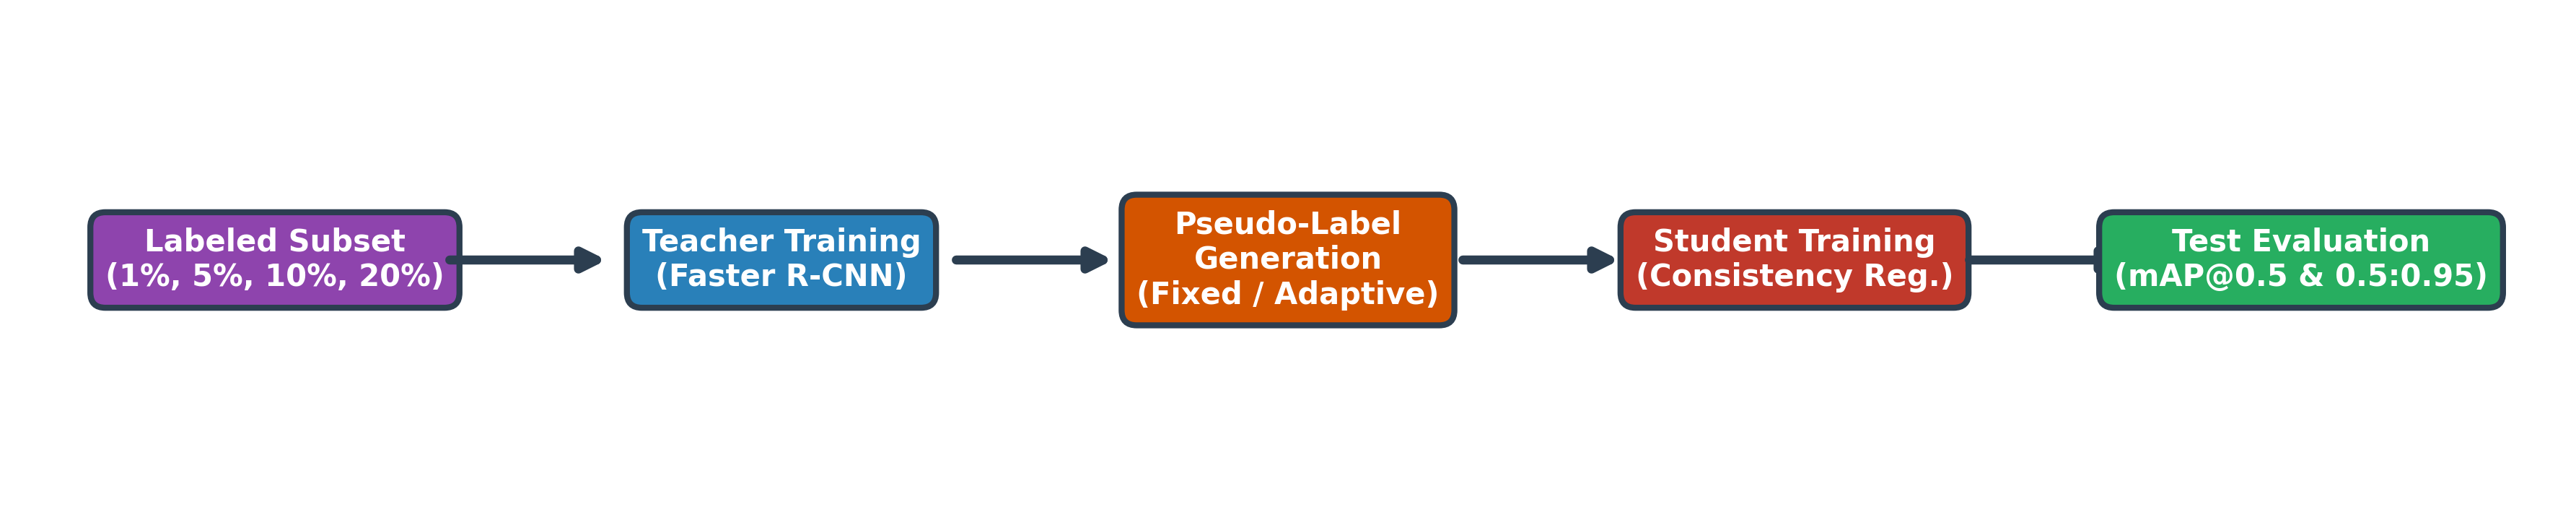
\includegraphics[width=\columnwidth]{fig1_workflow.png}
\caption{Overall workflow of the semi-supervised WBC detection framework. The labeled subset is used to train the teacher detector, pseudo-labels are generated on unlabeled images using fixed or adaptive confidence thresholding, the student detector is trained using labeled and pseudo-labeled samples, and final performance is evaluated on the test set.}
\label{fig:workflow}
\end{figure}

\subsection{Detection Models and Pseudo-Labeling Strategies}
The supervised baseline was Faster R-CNN with a MobileNetV3-Large FPN backbone. The detector was initialized with pretrained weights, and the classification head was replaced for single-class WBC detection. Since Faster R-CNN includes the background class internally, the number of output classes was set to two: background and WBC. The supervised baseline was trained only on the labeled subset for each annotation ratio.

The STAC-inspired framework consisted of three stages, as summarized in Fig.~\ref{fig:workflow}. First, a teacher detector was trained using only the labeled subset. Second, the trained teacher generated pseudo-labels on the unlabeled pool. Third, a student detector was trained using the union of the labeled subset and pseudo-labeled unlabeled images.

For fixed-threshold STAC, a confidence threshold of $\tau=0.85$ was used. Only predictions with confidence scores greater than or equal to this threshold were retained as pseudo-labels. For adaptive-threshold STAC, the threshold was computed from the distribution of teacher confidence scores:
\begin{equation}
\tau = \mathrm{clip}(\mu - 0.5\sigma, 0.50, 0.88),
\end{equation}
where $\mu$ and $\sigma$ are the mean and standard deviation of confidence scores collected from the unlabeled predictions.

The Soft Teacher-inspired framework used a student detector and an EMA teacher detector. The student was optimized using labeled images and pseudo-labeled unlabeled images. The teacher was updated from the student weights using:
\begin{equation}
\theta_T \leftarrow \alpha \theta_T + (1-\alpha)\theta_S,
\end{equation}
where $\theta_T$ represents teacher parameters, $\theta_S$ represents student parameters, and $\alpha$ is the EMA coefficient. The EMA coefficient was set to $\alpha=0.999$. Two threshold strategies were tested for Soft Teacher: fixed thresholding with $\tau=0.85$ and adaptive thresholding based on the confidence-score distribution.

The fixed and adaptive threshold values used in the experiments are summarized in Table~\ref{tab:thresholds}. For Soft Teacher adaptive thresholding, the values correspond to the final epoch thresholds.

\begin{table}[!t]
\caption{Fixed and adaptive confidence thresholds used for pseudo-label generation.}
\label{tab:thresholds}
\centering
\resizebox{\columnwidth}{!}{
\begin{tabular}{lcccc}
\toprule
\textbf{Method} & \textbf{1\%} & \textbf{5\%} & \textbf{10\%} & \textbf{20\%} \\
\midrule
STAC fixed & 0.85 & 0.85 & 0.85 & 0.85 \\
STAC adaptive & $\approx$0.52 & $\approx$0.58 & $\approx$0.72 & $\approx$0.81 \\
Soft Teacher fixed & 0.85 & 0.85 & 0.85 & 0.85 \\
Soft Teacher adaptive & $\approx$0.50 & $\approx$0.55 & $\approx$0.80 & $\approx$0.85 \\
\bottomrule
\end{tabular}
}
\end{table}

\subsection{Simplifications Relative to the Original STAC and Soft Teacher Methods}
The semi-supervised methods implemented in this study should be interpreted as STAC-inspired and Soft Teacher-inspired frameworks rather than exact reproductions of the original algorithms. This clarification is important because the original methods were designed and evaluated on large-scale general object detection benchmarks, while this study focuses on a small-scale, single-class medical detection problem.

In the STAC-inspired approach, the core offline pseudo-labeling idea was retained. A detector was first trained on the labeled subset, pseudo-labels were generated on the unlabeled pool, and a student detector was then trained using both labeled and pseudo-labeled data. However, several components of the original STAC pipeline were simplified. The full multi-stage training recipe, more complex consistency regularization strategies, unaligned bounding box matching, and bounding box regression consistency loss were not reproduced. Instead, this study used a confidence-threshold-based pseudo-label filtering strategy and standard PyTorch Faster R-CNN updates adapted to single-class WBC detection.

Similarly, the Soft Teacher-inspired approach retained the main EMA teacher-student mechanism but simplified several components of the original method. The original box jittering strategy, multiple classification thresholds for background sample selection, and regression-variance-based box filtering were not implemented. The method was adapted to a fixed image size, limited batch size, and single-class WBC detection setting. Pseudo-labels were selected using a single confidence-score filter, and the teacher model was updated using EMA with $\alpha=0.999$.

\subsection{Evaluation Metrics}
Final detection performance was evaluated using mAP@0.5, mAP@0.5:0.95, precision, recall, and F1-score. Precision, recall, and F1-score were computed as follows:
\begin{equation}
Precision = \frac{TP}{TP + FP},
\end{equation}
\begin{equation}
Recall = \frac{TP}{TP + FN},
\end{equation}
\begin{equation}
F1 = \frac{2 \times Precision \times Recall}{Precision + Recall}.
\end{equation}
In WBC detection, recall is especially important because false negatives correspond to missed WBC regions that cannot be recovered by downstream classification or morphological analysis.

In addition to final test performance, pseudo-label quality was evaluated separately. A pseudo-label was considered a true positive if its Intersection over Union (IoU) with a ground-truth WBC box was at least 0.5. IoU was computed as:
\begin{equation}
IoU = \frac{B_p \cap B_g}{B_p \cup B_g},
\end{equation}
where $B_p$ is the predicted box and $B_g$ is the ground-truth box. Pseudo-label precision, recall, and F1-score were then calculated from true positive, false positive, and false negative pseudo-label matches.

\section{Experimental Setup}
All experiments were implemented in Python using PyTorch and TorchVision. The TXL-PBC dataset was loaded using its official train, validation, and test folders. Images were resized to $416 \times 416$ in production mode. The random seed was fixed to 42 for all data splitting and initialization steps.

The model was trained using stochastic gradient descent with a learning rate of 0.005, momentum of 0.9, and weight decay of 0.0005. The batch size was set to 4. Gradient clipping was applied for training stability. The supervised Faster R-CNN baseline was trained for 15 epochs. In the STAC-inspired setting, the teacher detector was trained for 10 epochs and the student detector was trained for 15 epochs. In the Soft Teacher-inspired setting, joint teacher-student training was performed for 15 epochs.

Weak and strong augmentation strategies were used in the semi-supervised training pipeline. Augmentation is commonly used to improve model robustness under limited data conditions \cite{shorten2019augmentation}. In this study, weak augmentation mainly involved spatial flipping, while strong augmentation additionally involved photometric perturbations such as brightness variation, blur, noise, and cutout-style occlusion.

For each annotation ratio, five configurations were evaluated:
\begin{itemize}
    \item Faster R-CNN supervised baseline,
    \item STAC-inspired training with fixed threshold,
    \item STAC-inspired training with adaptive threshold,
    \item Soft Teacher-inspired training with fixed threshold,
    \item Soft Teacher-inspired training with adaptive threshold.
\end{itemize}

The implementation code was uploaded to a public GitHub repository and cited in the references section \cite{githubrepo}.

\section{Results and Discussion}

\subsection{Detection Performance under Different Annotation Ratios}
Table~\ref{tab:map50} presents the mAP@0.5 results across all annotation ratios. The supervised Faster R-CNN baseline achieved 0.9634 mAP@0.5 even with only 1\% labeled data. This indicates that the WBC class in TXL-PBC is visually distinctive enough for the pretrained detector to learn a strong localization model from a very small labeled subset.

\begin{table}[!t]
\caption{Test mAP@0.5 results across labeled-data fractions.}
\label{tab:map50}
\centering
\resizebox{\columnwidth}{!}{
\begin{tabular}{lcccc}
\toprule
\textbf{Method} & \textbf{1\%} & \textbf{5\%} & \textbf{10\%} & \textbf{20\%} \\
\midrule
Faster R-CNN baseline & 0.9634 & \textbf{0.9850} & 0.9848 & 0.9848 \\
STAC fixed & 0.9632 & 0.9841 & \textbf{0.9850} & 0.9849 \\
STAC adaptive & \textbf{0.9644} & 0.9849 & \textbf{0.9850} & \textbf{0.9850} \\
Soft Teacher fixed & 0.8477 & 0.9821 & \textbf{0.9850} & \textbf{0.9850} \\
Soft Teacher adaptive & 0.8322 & 0.9704 & \textbf{0.9850} & \textbf{0.9850} \\
\bottomrule
\end{tabular}
}
\end{table}

At 1\% labeled data, STAC adaptive achieved the highest mAP@0.5 value with 0.9644, but the improvement over the supervised baseline was small. In contrast, both Soft Teacher configurations performed worse than the supervised baseline in the 1\% setting. This suggests that online pseudo-labeling may become unstable when the initial labeled subset is too small.

Fig.~\ref{fig:sensitivity} visualizes the sensitivity of final mAP@0.5 performance to the labeled-data fraction and pseudo-label thresholding strategy. The curve shows that most methods reached high mAP@0.5 once at least 5\% of the training set was labeled, whereas Soft Teacher-based training was more sensitive under the 1\% setting. This supports the interpretation that teacher-student pseudo-labeling requires a sufficiently reliable initial teacher model.

\begin{figure}[!t]
\centering
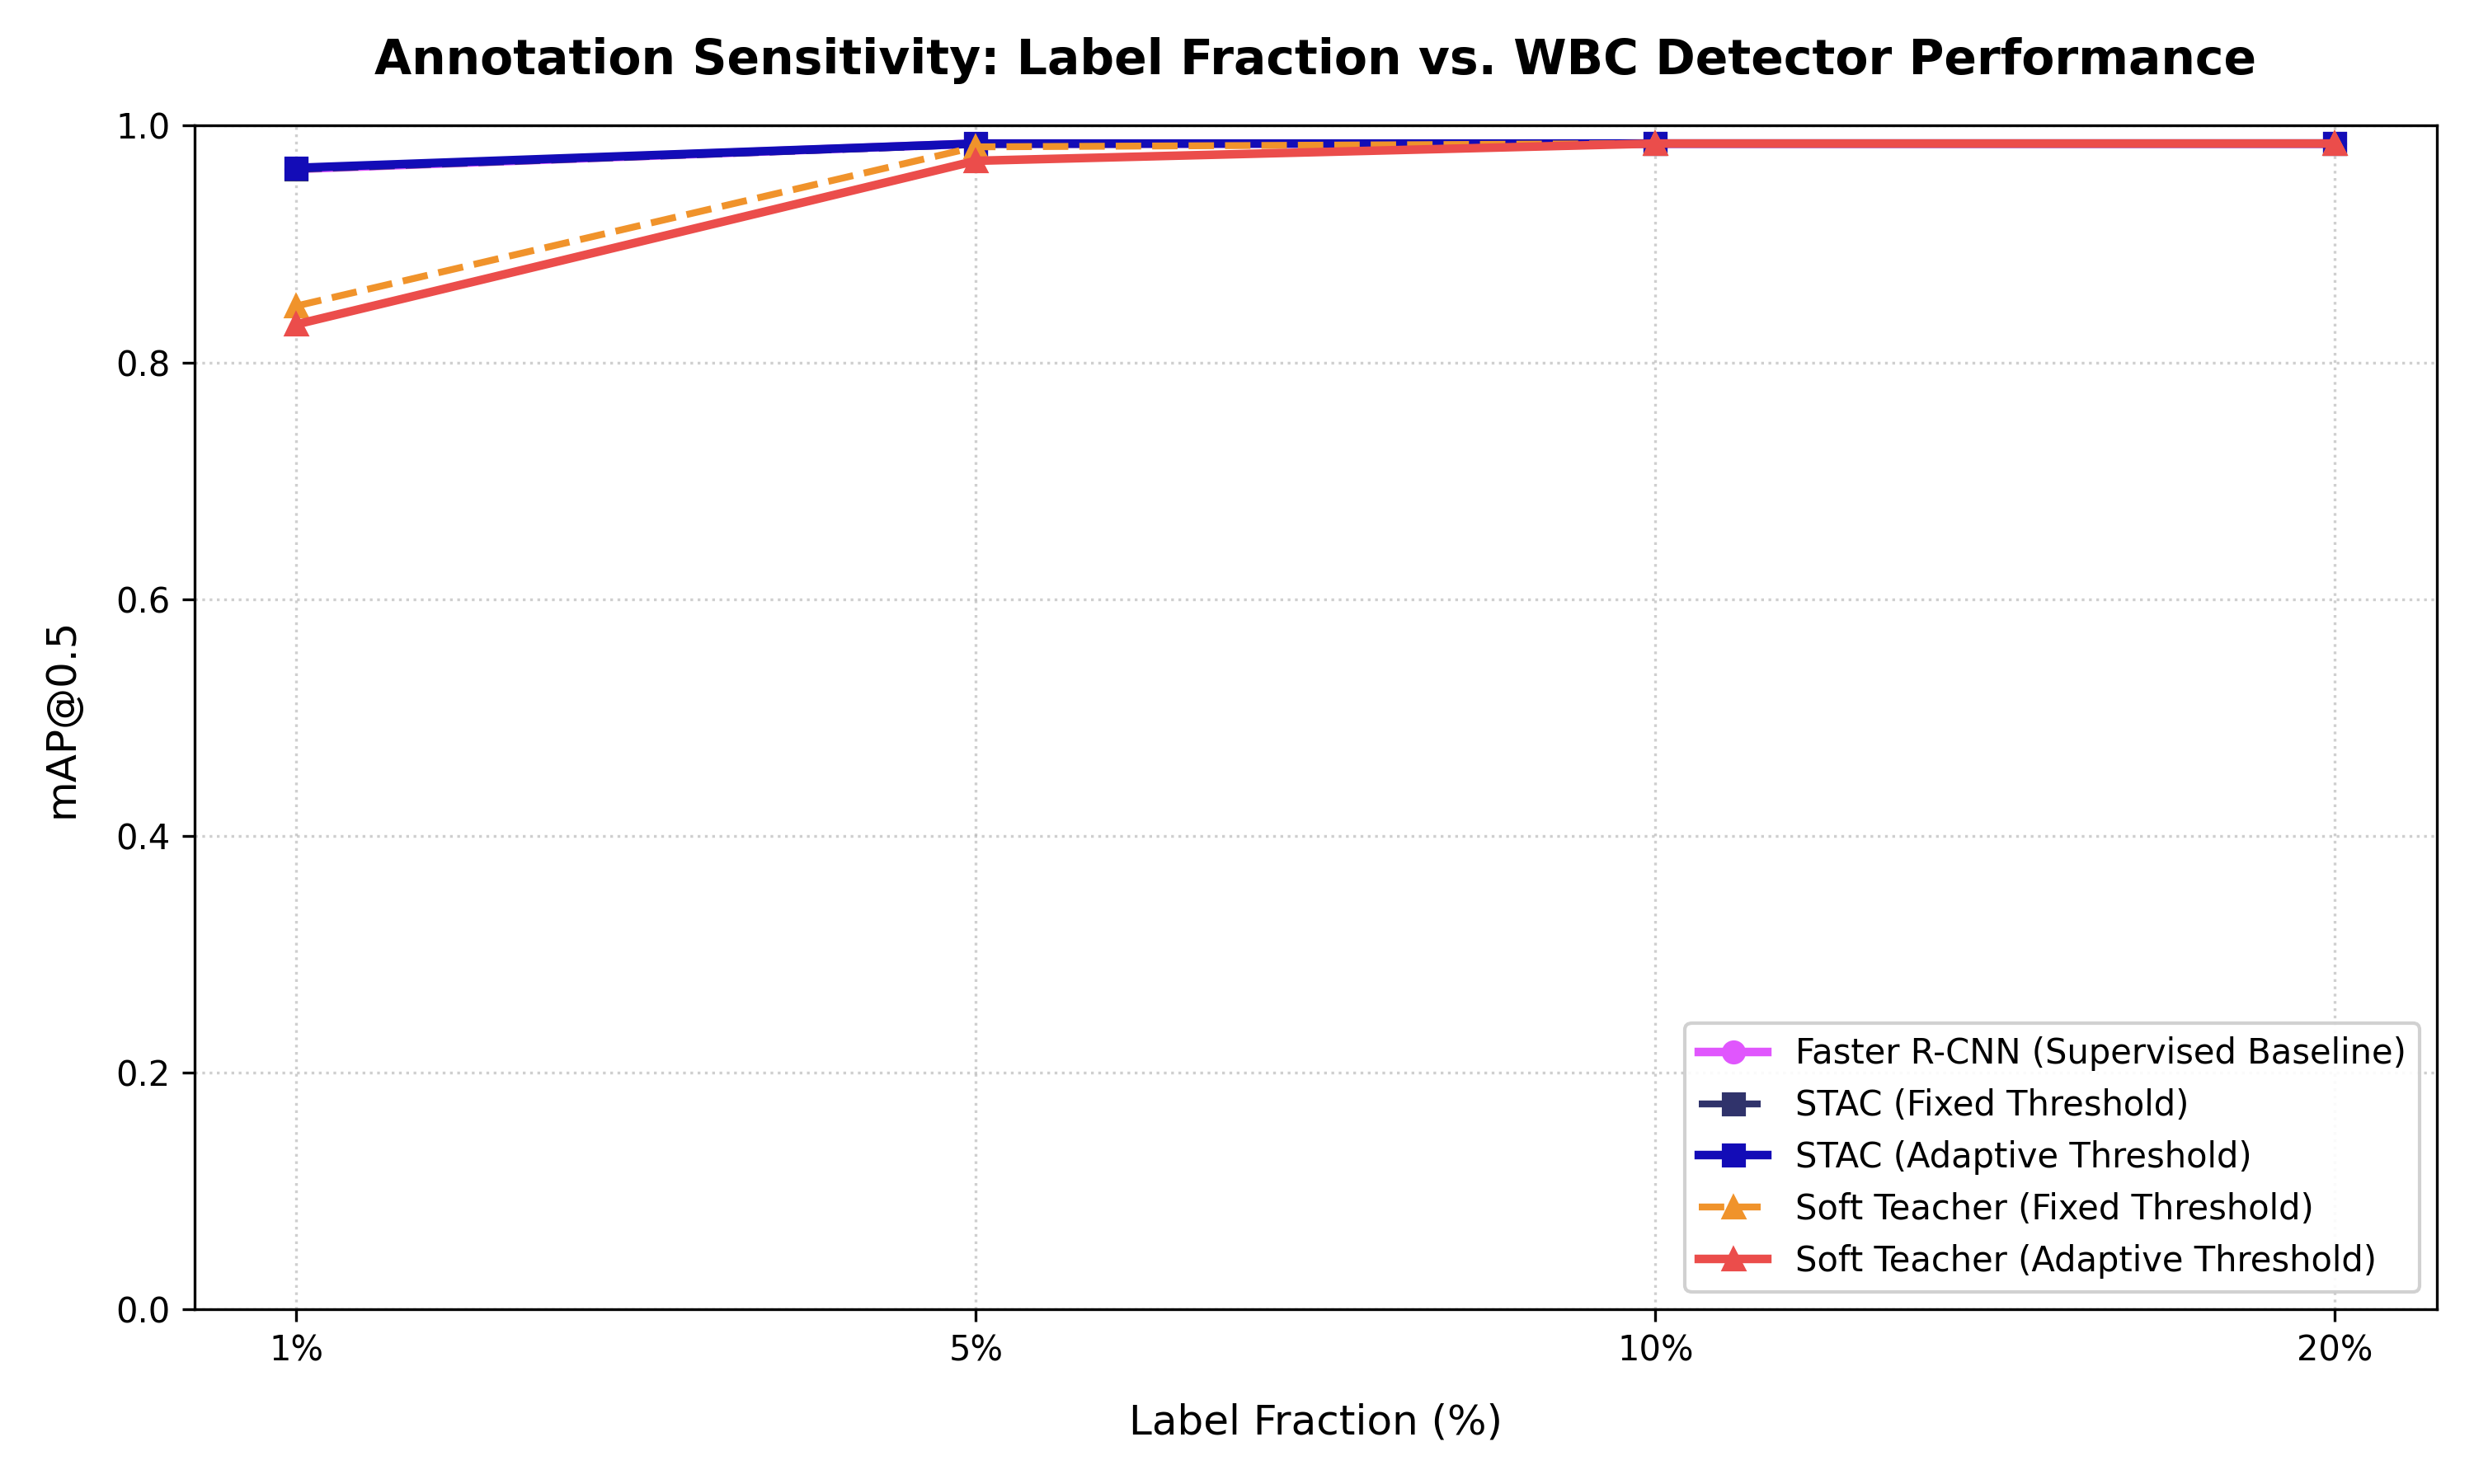
\includegraphics[width=\columnwidth]{sensitivity_comparison.png}
\caption{Sensitivity comparison of final detection performance across labeled-data fractions. The plot shows mAP@0.5 trends for the supervised baseline, STAC-inspired methods, and Soft Teacher-inspired methods under fixed and adaptive thresholding strategies.}
\label{fig:sensitivity}
\end{figure}

Table~\ref{tab:map5095} shows the mAP@0.5:0.95 results. This metric is more sensitive to bounding box localization quality because it averages AP values across multiple IoU thresholds.

\begin{table}[!t]
\caption{Test mAP@0.5:0.95 results across labeled-data fractions.}
\label{tab:map5095}
\centering
\resizebox{\columnwidth}{!}{
\begin{tabular}{lcccc}
\toprule
\textbf{Method} & \textbf{1\%} & \textbf{5\%} & \textbf{10\%} & \textbf{20\%} \\
\midrule
Faster R-CNN baseline & \textbf{0.7148} & 0.7189 & 0.7358 & 0.8118 \\
STAC fixed & 0.5761 & 0.6578 & 0.7673 & 0.8022 \\
STAC adaptive & 0.6354 & \textbf{0.7205} & 0.7555 & 0.7567 \\
Soft Teacher fixed & 0.4669 & 0.6891 & 0.7136 & 0.7406 \\
Soft Teacher adaptive & 0.2737 & 0.6465 & \textbf{0.8133} & \textbf{0.8323} \\
\bottomrule
\end{tabular}
}
\end{table}

The mAP@0.5:0.95 results reveal differences that were not clearly visible in the mAP@0.5 table. In the 1\% setting, the supervised baseline achieved the best localization quality with 0.7148. This means that adding pseudo-labels did not improve strict localization when only 8 labeled images were available. At 10\% and 20\% labeled data, Soft Teacher adaptive achieved the highest mAP@0.5:0.95 values, reaching 0.8133 and 0.8323, respectively. This suggests that the teacher-student mechanism becomes useful once the teacher model is sufficiently reliable.

To complement mAP-based evaluation, final detection precision, recall, and F1-score were also reported. These metrics provide a clearer interpretation of false positives and missed WBCs, which is particularly important in medical image analysis. The final test precision, recall, and F1-score values are presented in Tables~\ref{tab:precision}, \ref{tab:recall}, and \ref{tab:f1}, respectively.

\begin{table}[!t]
\caption{Final test precision across labeled-data fractions.}
\label{tab:precision}
\centering
\resizebox{\columnwidth}{!}{
\begin{tabular}{lcccc}
\toprule
\textbf{Method} & \textbf{1\%} & \textbf{5\%} & \textbf{10\%} & \textbf{20\%} \\
\midrule
Faster R-CNN baseline & 0.9275 & 1.0000 & 0.9850 & 0.9848 \\
STAC fixed & 0.9846 & 0.9353 & 0.9924 & 1.0000 \\
STAC adaptive & 0.9773 & 0.9776 & 0.9924 & 1.0000 \\
Soft Teacher fixed & 0.9365 & 0.9922 & 1.0000 & 1.0000 \\
Soft Teacher adaptive & 0.1527 & 0.3696 & 0.9924 & 1.0000 \\
\bottomrule
\end{tabular}
}
\end{table}

\begin{table}[!t]
\caption{Final test recall across labeled-data fractions.}
\label{tab:recall}
\centering
\resizebox{\columnwidth}{!}{
\begin{tabular}{lcccc}
\toprule
\textbf{Method} & \textbf{1\%} & \textbf{5\%} & \textbf{10\%} & \textbf{20\%} \\
\midrule
Faster R-CNN baseline & 0.9624 & 0.9624 & 0.9850 & 0.9774 \\
STAC fixed & 0.9624 & 0.9774 & 0.9850 & 0.9774 \\
STAC adaptive & 0.9699 & 0.9850 & 0.9850 & 0.9850 \\
Soft Teacher fixed & 0.4436 & 0.9549 & 0.9699 & 0.9774 \\
Soft Teacher adaptive & 0.9699 & 0.9699 & 0.9850 & 0.9850 \\
\bottomrule
\end{tabular}
}
\end{table}

\begin{table}[!t]
\caption{Final test F1-score across labeled-data fractions.}
\label{tab:f1}
\centering
\resizebox{\columnwidth}{!}{
\begin{tabular}{lcccc}
\toprule
\textbf{Method} & \textbf{1\%} & \textbf{5\%} & \textbf{10\%} & \textbf{20\%} \\
\midrule
Faster R-CNN baseline & 0.9446 & 0.9808 & 0.9850 & 0.9811 \\
STAC fixed & 0.9734 & 0.9559 & 0.9887 & 0.9886 \\
STAC adaptive & 0.9736 & 0.9813 & 0.9887 & 0.9924 \\
Soft Teacher fixed & 0.6020 & 0.9732 & 0.9847 & 0.9886 \\
Soft Teacher adaptive & 0.2638 & 0.5353 & 0.9887 & 0.9924 \\
\bottomrule
\end{tabular}
}
\end{table}

The precision and recall results support the interpretation of the mAP scores. In the 1\% and 5\% settings, Soft Teacher adaptive produced low precision values of 0.1527 and 0.3696, respectively, indicating that the model accepted a considerable number of false-positive pseudo-labels when the adaptive threshold was permissive. Although its recall remained high in these settings, the low F1-scores of 0.2638 and 0.5353 show that recall alone was not sufficient for reliable detection. In addition, Soft Teacher fixed produced a low recall value of 0.4436 and an F1-score of 0.6020 in the 1\% setting, suggesting that the high fixed threshold caused label starvation by rejecting many potentially useful predictions. In contrast, Soft Teacher adaptive achieved strong F1-scores at 10\% and 20\% labeled data, reaching 0.9887 and 0.9924, respectively. This confirms that the same teacher-student mechanism becomes more effective once the labeled subset is sufficiently informative.

\subsection{Pseudo-Label Quality and Threshold Sensitivity}
Table~\ref{tab:plf1} presents pseudo-label F1-scores for the semi-supervised methods. This analysis is important because high final detection performance does not necessarily mean that pseudo-labels were reliable. Evaluating pseudo-label quality separately helps identify whether performance degradation comes from poor pseudo-label generation or from student training behavior.

\begin{table}[!t]
\caption{Pseudo-label F1-score across labeled-data fractions.}
\label{tab:plf1}
\centering
\resizebox{\columnwidth}{!}{
\begin{tabular}{lcccc}
\toprule
\textbf{Method} & \textbf{1\%} & \textbf{5\%} & \textbf{10\%} & \textbf{20\%} \\
\midrule
STAC fixed & \textbf{0.9608} & 0.9629 & 0.9809 & \textbf{0.9903} \\
STAC adaptive & 0.9461 & \textbf{0.9837} & \textbf{0.9847} & 0.9875 \\
Soft Teacher fixed & 0.0000 & 0.0115 & 0.0000 & 0.0000 \\
Soft Teacher adaptive & 0.2603 & 0.5157 & 0.9829 & 0.9896 \\
\bottomrule
\end{tabular}
}
\end{table}

Fig.~\ref{fig:pseudoquality} provides a visual comparison of pseudo-label quality under fixed and adaptive thresholding. The plot highlights how pseudo-label precision and recall change across labeled-data fractions and helps explain the two main low-label failure mechanisms observed in this study. Strict thresholding can reduce pseudo-label coverage and cause label starvation, whereas permissive adaptive thresholding can increase recall while also introducing false-positive pseudo-labels.

\begin{figure}[!t]
\centering
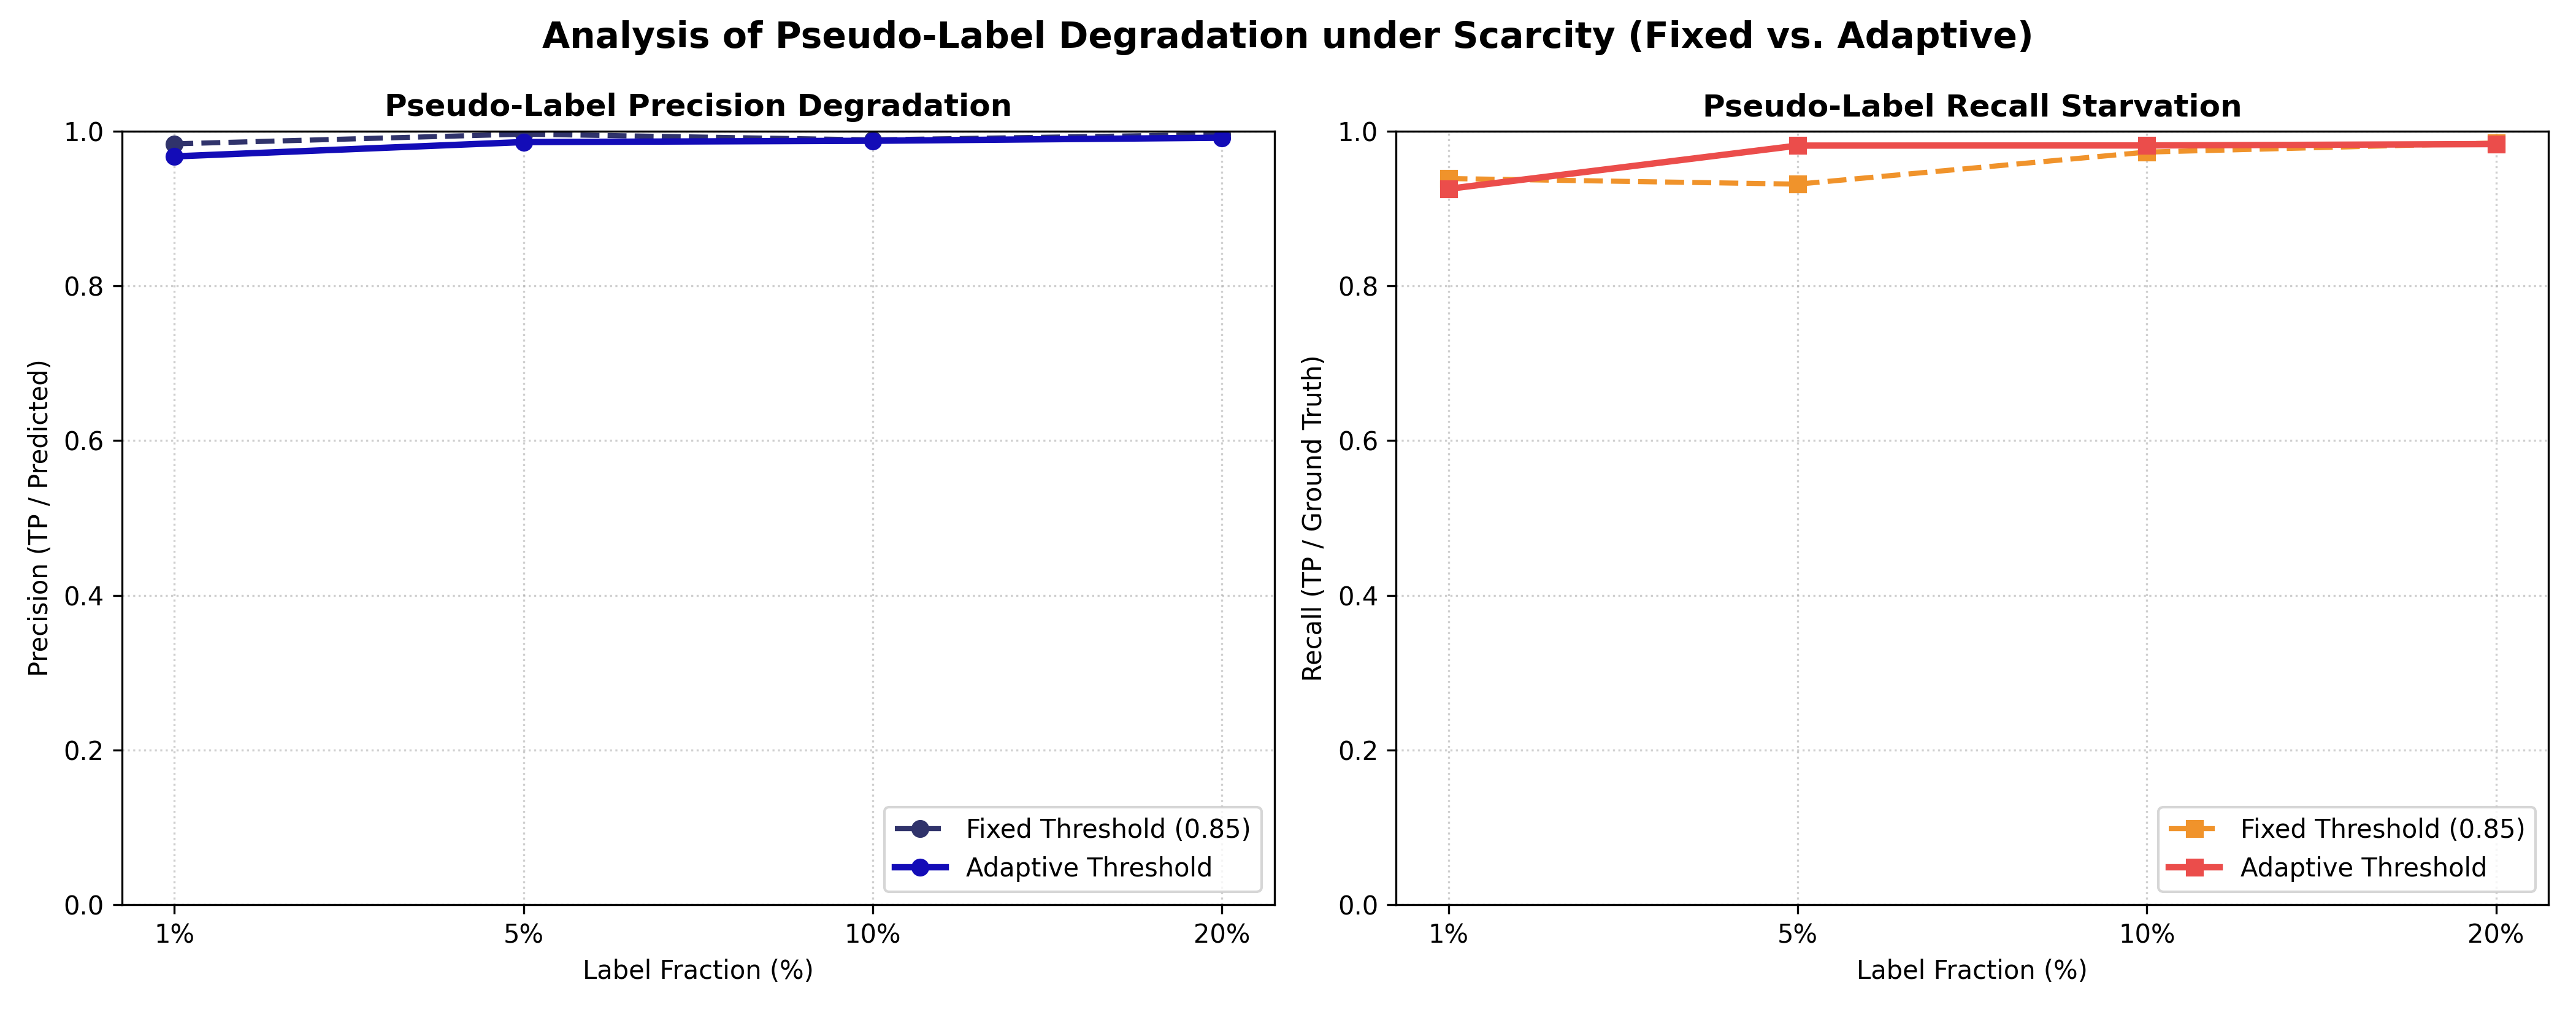
\includegraphics[width=\columnwidth]{pseudo_label_quality.png}
\caption{Pseudo-label quality analysis across labeled-data fractions. The plot compares pseudo-label precision and recall under fixed and adaptive thresholding strategies and illustrates the relationship between pseudo-label coverage, label starvation, and noise propagation.}
\label{fig:pseudoquality}
\end{figure}

STAC generated stable pseudo-labels across all annotation ratios. Even at 1\% labeled data, STAC fixed achieved a pseudo-label F1-score of 0.9608. This indicates that the fixed threshold of 0.85 selected fewer but more reliable predictions. STAC adaptive achieved lower F1 at 1\%, but it improved at 5\% and 10\%, showing that adaptive thresholding became more effective when the teacher had access to more labeled examples.

Soft Teacher showed a different behavior. In the 1\% and 5\% settings, Soft Teacher adaptive produced higher coverage but low pseudo-label quality. This indicates that it accepted many uncertain boxes as pseudo-labels, increasing false positives. At 10\% and 20\%, however, Soft Teacher adaptive produced strong pseudo-labels with F1-scores of 0.9829 and 0.9896. This explains why it achieved the best mAP@0.5:0.95 at these annotation ratios.

\subsection{Error Analysis under Extreme Annotation Scarcity}
The results show that pseudo-labeling is not always beneficial in extremely low-label regimes. When only 1\% of the training set was labeled, the teacher model was trained on only a few WBC examples. In such a case, the detector may not learn enough appearance variation and may produce overconfident but incorrect predictions. If these predictions are used as pseudo-labels, the student model can learn from false positives or poorly localized boxes.

Two failure modes were observed. The first is \textit{label starvation}. With a high fixed threshold, the model may reject most predictions, causing the unlabeled pool to contribute little or no useful training signal. This behavior was observed in Soft Teacher fixed, where pseudo-label F1 was 0.0000 in several settings and final recall was low in the 1\% setting. The second failure mode is \textit{noise propagation}. With a permissive adaptive threshold, the model may accept too many uncertain boxes, increasing pseudo-label recall but decreasing precision. This was observed in Soft Teacher adaptive at 1\% and 5\% labeled data, where final precision values were low and final mAP@0.5 was lower than the supervised baseline.

A third related failure mode is \textit{poor localization}. In this case, the WBC region may be partially detected, but the accepted pseudo-label box has insufficient overlap with the ground-truth annotation. These poorly localized boxes can degrade localization learning in the student model, especially under low-label conditions.

\subsection{Qualitative Detection Examples and Failure Cases}
Fig.~\ref{fig:samples} presents representative WBC detection outputs from the TXL-PBC test set. Green boxes indicate ground-truth WBC annotations, while red boxes indicate predicted bounding boxes with confidence scores. The examples show that the detector can localize WBCs accurately under different cell morphologies, nuclear appearances, and surrounding red blood cell distributions.

\begin{figure}[!t]
\centering
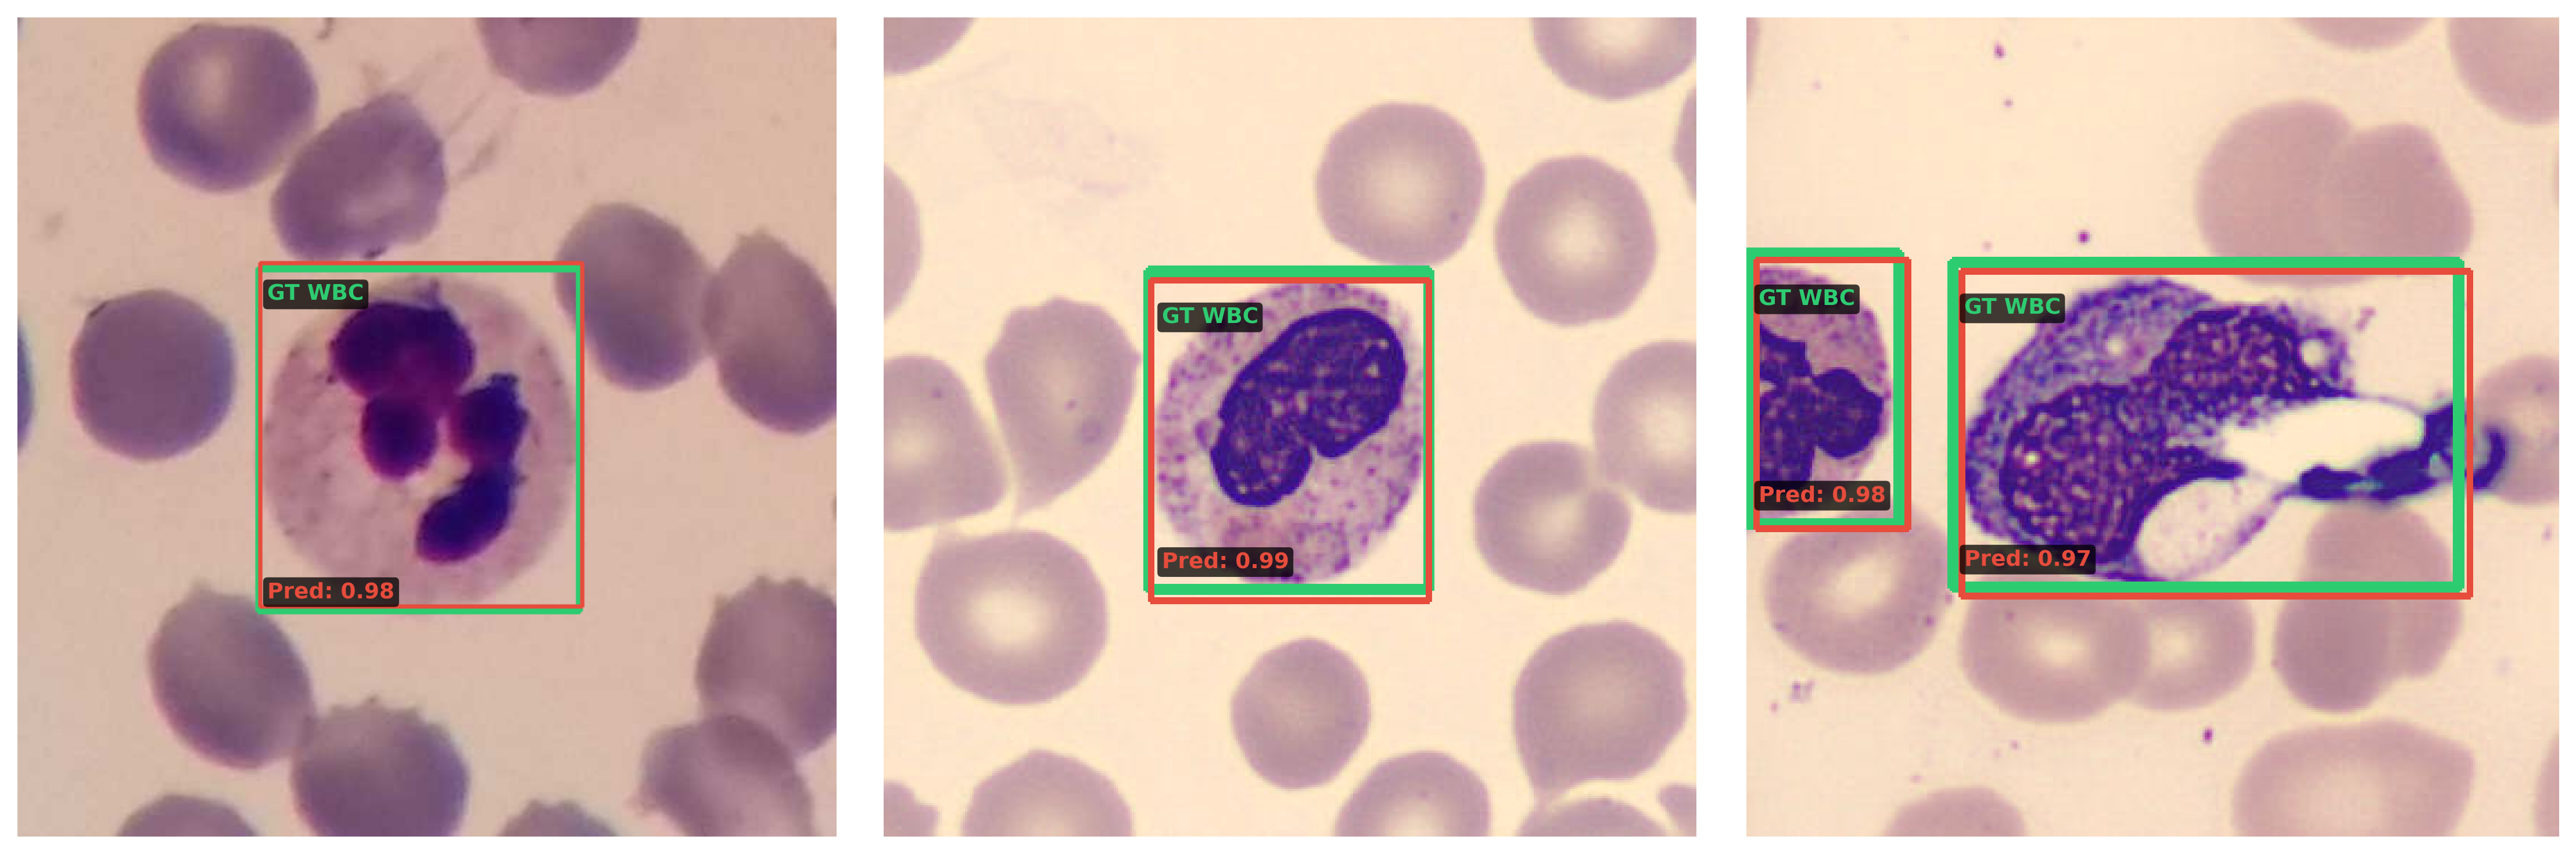
\includegraphics[width=\columnwidth]{fig2_detection_examples.png}
\caption{Representative successful WBC detection examples from the TXL-PBC test set. Green boxes indicate ground-truth WBC annotations, while red boxes indicate predicted WBC bounding boxes with confidence scores.}
\label{fig:samples}
\end{figure}

Fig.~\ref{fig:failures} shows representative failure cases for the Soft Teacher-inspired model under the 1\% and 5\% labeled-data settings. These examples support the quantitative findings and illustrate why pseudo-labeling may degrade performance under extreme annotation scarcity. Fig.~\ref{fig:failures}(a) shows label starvation, where the high fixed threshold rejected useful predictions and caused a missed WBC. Fig.~\ref{fig:failures}(b) shows noise propagation, where a low adaptive threshold accepted a false-positive pseudo-label from a non-WBC region. Fig.~\ref{fig:failures}(c) shows poor localization, where a shifted bounding box with insufficient IoU was accepted as a pseudo-label and could therefore weaken box-regression learning.

\begin{figure}[!t]
\centering
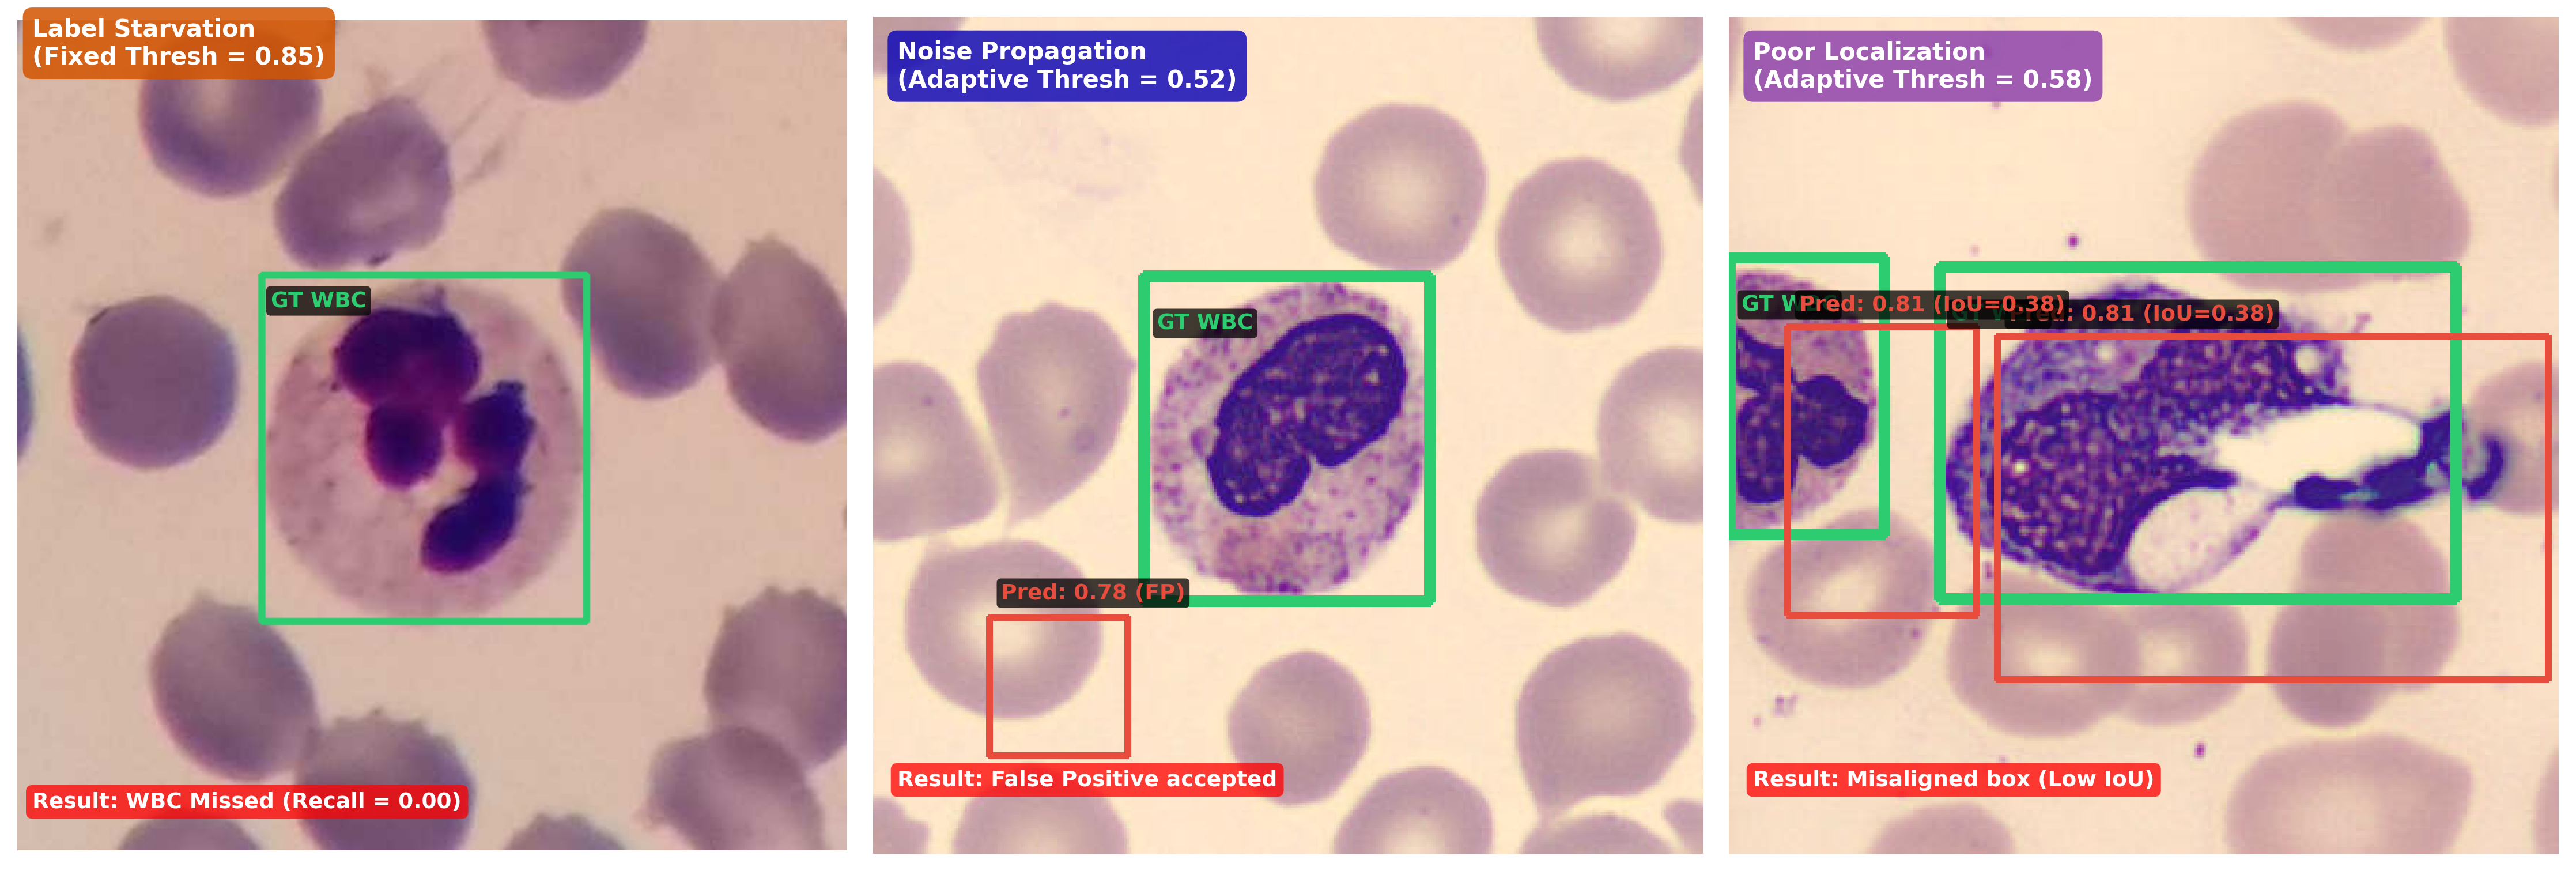
\includegraphics[width=\columnwidth]{fig3_failures.png}
\caption{Representative Soft Teacher failure cases under annotation scarcity. (a) Label starvation caused by a high fixed threshold ($\tau=0.85$), resulting in a missed WBC. (b) Noise propagation caused by a permissive adaptive threshold ($\tau\approx0.50$), where a non-WBC region is accepted as a false-positive pseudo-label. (c) Poor localization, where a shifted bounding box with insufficient IoU is accepted as a pseudo-label.}
\label{fig:failures}
\end{figure}

\FloatBarrier

\section{Conclusion}
This study evaluated semi-supervised WBC detection under limited bounding box annotations using the TXL-PBC dataset. Faster R-CNN was used as a supervised baseline, while STAC-inspired and Soft Teacher-inspired semi-supervised frameworks were compared under 1\%, 5\%, 10\%, and 20\% labeled-data settings.

The results showed that the supervised Faster R-CNN baseline achieved high mAP@0.5 even with only 1\% labeled data. Therefore, semi-supervised learning did not consistently improve mAP@0.5 in all settings. However, stricter localization metrics, final precision-recall-F1 analysis, and pseudo-label quality evaluation revealed important differences. STAC produced stable pseudo-labels across all label fractions, while Soft Teacher adaptive was unstable under 1\% and 5\% labeled data but achieved the best localization quality at 10\% and 20\%.

The results suggest that semi-supervised WBC detection is strongly affected by the reliability of the teacher model and the pseudo-label thresholding strategy. In extremely low-label settings, pseudo-labeling may cause label starvation, noise propagation, or poor localization. However, when a sufficiently informative labeled subset is available, adaptive teacher-student training can improve localization quality.

The main limitation of this study is that the task was simplified to single-class WBC detection. RBC and platelet detection were not included in the final evaluation. In addition, the implemented STAC and Soft Teacher frameworks were simplified versions inspired by the original methods, rather than full official reproductions. Future work should extend the analysis to multi-class blood cell detection, test additional backbones, repeat experiments with multiple random seeds, and evaluate the approach on external blood smear datasets.

\section*{Acknowledgment}
The author used AI-assisted tools during the preparation of this study for language editing, organization of the paper structure, LaTeX formatting support, and improving the clarity of the discussion. The experimental design, implementation, numerical results, interpretation, and final responsibility for the paper belong to the author.

\begin{thebibliography}{00}

\bibitem{ren2015faster}
S. Ren, K. He, R. Girshick, and J. Sun, ``Faster R-CNN: Towards real-time object detection with region proposal networks,'' in \textit{Advances in Neural Information Processing Systems}, vol. 28, pp. 91--99, 2015.

\bibitem{gan2025txlpbc}
L. Gan, X. Li, and X. Wang, ``A curated and re-annotated peripheral blood cell dataset integrating four public resources,'' \textit{Scientific Data}, vol. 12, article no. 1694, 2025, doi: 10.1038/s41597-025-05980-z.

\bibitem{sohn2020stac}
K. Sohn, Z. Zhang, C.-L. Li, H. Zhang, C.-Y. Lee, and T. Pfister, ``A simple semi-supervised learning framework for object detection,'' \textit{arXiv preprint arXiv:2005.04757}, 2020.

\bibitem{xu2021softteacher}
M. Xu, Z. Zhang, H. Hu, J. Wang, L. Wang, F. Wei, X. Bai, and Z. Liu, ``End-to-end semi-supervised object detection with Soft Teacher,'' in \textit{Proceedings of the IEEE/CVF International Conference on Computer Vision (ICCV)}, pp. 3060--3069, 2021.

\bibitem{tarvainen2017meanteacher}
A. Tarvainen and H. Valpola, ``Mean teachers are better role models: Weight-averaged consistency targets improve semi-supervised deep learning results,'' in \textit{Advances in Neural Information Processing Systems}, vol. 30, pp. 1195--1204, 2017.

\bibitem{sohn2020fixmatch}
K. Sohn, D. Berthelot, C.-L. Li, Z. Zhang, N. Carlini, E. D. Cubuk, A. Kurakin, H. Zhang, and C. Raffel, ``FixMatch: Simplifying semi-supervised learning with consistency and confidence,'' in \textit{Advances in Neural Information Processing Systems}, vol. 33, pp. 596--608, 2020.

\bibitem{liu2021unbiasedteacher}
Y.-C. Liu, C.-Y. Ma, Z. He, C.-W. Kuo, K. Chen, P. Zhang, B. Wu, Z. Kira, and P. Vajda, ``Unbiased Teacher for semi-supervised object detection,'' in \textit{International Conference on Learning Representations}, 2021.

\bibitem{shorten2019augmentation}
C. Shorten and T. M. Khoshgoftaar, ``A survey on image data augmentation for deep learning,'' \textit{Journal of Big Data}, vol. 6, article no. 60, 2019, doi: 10.1186/s40537-019-0197-0.

\bibitem{githubrepo}
F. Yal\c{c}\i n, ``Semi-supervised WBC detection implementation,'' GitHub repository, 2026. [Online]. Available: \url{https://github.com/fdmylcn/WBC_Detection_ECE664}

\end{thebibliography}

\end{document}
